\section{Passo 6 — Triagem, etapa 2, e classificação por estrato}
\label{sec:passo6}

\subsection*{Objetivo}
Classificar as famílias mantidas por segmento de aplicação e por estrato analítico, produzindo a base
final do estudo.

\begin{figure}[H]
\centering
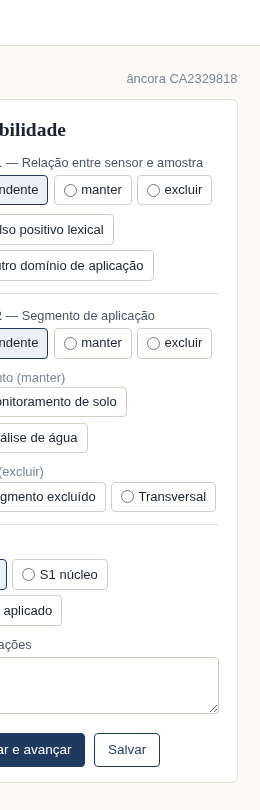
\includegraphics[width=0.4\linewidth]{img/08_triagem_painel.png}
\caption{Painel de decisão da ficha, recortado: etapa 1, etapa 2, estrato e observações.}
\label{fig:triagem2}
\end{figure}

\subsection*{O que fazer}
\begin{enumerate}
\item Clique em \textbf{Triar etapa 2}. Só aparecem as famílias mantidas na etapa 1.
\item Escolha o \textbf{segmento} de aplicação e, se houver, o motivo de exclusão da etapa 2.
\item Atribua o \textbf{estrato} (S1, S2, conforme a definição do estudo).
\item Registre observações quando a decisão não for óbvia; elas ficam na planilha.
\end{enumerate}

\subsection*{Como interpretar}
A etapa 2 responde ``para que serve a invenção?''; o estrato responde ``qual é o papel do tema na
invenção?''. São perguntas diferentes e não devem ser confundidas.

Na demonstração, S1 é ``o sensor é o objeto da invenção'' e S2 é ``o sensor é instrumento de um método
para outra finalidade''. A definição textual importa: sem ela, dois avaliadores classificam o mesmo
documento de formas diferentes.

\begin{nota}[Por que estratificar]
A média do corpus mistura invenções de naturezas distintas. Separar S1 e S2 permite comparar, por
exemplo, depositantes que protegem o componente e depositantes que protegem o método de uso --- e
evita conclusões sobre ``o setor'' a partir de populações heterogêneas.
\end{nota}

\begin{alerta}[Erro comum]
Deixar o estrato em branco e seguir para os indicadores. A base final fica incompleta e os gráficos
por estrato perdem parte das famílias sem aviso.
\end{alerta}

\subsection*{Checkpoint}
\marcador\; O PRISMA mostra a base final com o total de incluídas e a distribuição por estrato; não há
pendentes nas etapas 1 e 2.
